\chapter{Reading data from peripherals} \label{ch:ReadSwitch}
\chapterquote{Selfness for all brings about undisturbed harmony without loss of discrimination, and unshakable peace without indifference to the surroundings. }{Meher Baba}

\graphicspath{{Chapters/NiosReadSwitch/Figures/}}
\lstinputpath{Codes-Verilog/Chapter-Reading-Data-From-Peripherals} %path is defined in mypreamble


\section{Introduction}
In Chapter \ref{ch:NiosOverview}, the values of the variables in the code i.e. `led\_pattern' were sent to PIO (peripheral input/output) device  i.e. LED. In this chapter, we will learn to read the values from the PIO. More specifically, the values will be read from the external switches. These values will decide the blinking rate of the LED. Further, we will not create a new `.qsys' file, but modify the previous `.qsys' file to generate the new system. Also, we will see the procedures to modify the existing Nios project i.e. BSP and Application files (instead of creating the new project). 

\section{Modify Qsys file}\label{sec:ModifyQysFile}
First create or open a Quartus project as discussed in Chapter \ref{ch:NiosOverview}. Then open the `Qsys' file, which we have created in the previous chapter and modify the file as below, 
\begin{enumerate}
	\item \textbf{Modify LED port}: Double click on the `led' and change the `Width' column to `2' from `1'; because in this chapter, we will use two LEDs which will blink alternatively. 
	\item \textbf{Add Switch Port}: Next, add a new PIO device and set it to `output' port with width `8' as shown in Fig. \ref{fig:AddSwitch}. Next, rename it to `switch' and modify it's clock, reset and external connections as shown in Fig. \ref{fig:SwitchConnection}. 
	
	\begin{figure}[!h]
		\centering
		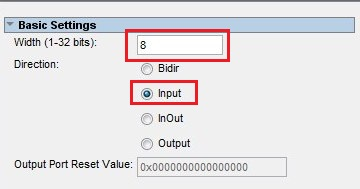
\includegraphics[scale=0.65]{AddSwitch}
		\caption{Add switch of width 8}
		\label{fig:AddSwitch}
	\end{figure}
	\begin{figure}[!h]
		\centering
		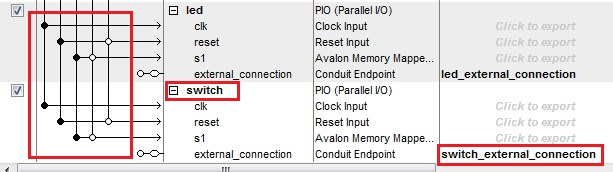
\includegraphics[scale=0.65]{SwitchConnection}
		\caption{Rename and Modify the port for Switch}
		\label{fig:SwitchConnection}
	\end{figure}
	\item Next, assign base address by clicking on System$\rightarrow$Assign base addresses. 
	\item Finally, generate the system, by clicking on the `Generate button' with correct simulation settings, as shown in Fig. \ref{fig:SystemGeneated}.
\end{enumerate} 

\section{Modify top level design in Quartus}
Since, LED port is modified and the `switch' port is added to the system, therefore top level module should be modified to assign proper connections to the FPGA chip. Top level design for this purpose is shown in Listing \ref{verilog:blinkingLED_VisualTestCh2}.
\lstinputlisting[
caption    = {Modify top level design in Quartus},
language = Verilog,
label      = {verilog:blinkingLED_VisualTestCh2}
]{VerilogCodes/blinkingLED_VisualTest.v}

\section{Modify  Nios project}
Since `Qsys' system is modified, therefore corresponding `.sopcinfo' file is modified also. Now, we need to update the system according to the new `.sopcinfo' file. 

\subsection{Adding Nios project to workspace}
If `workspace is changed' or `BSP/Application files are removed' from the current workspace, then we need to add these files again in the project, as discussed below, 
\begin{enumerate}
	\item First go to Files$\rightarrow$Import$\rightarrow$`Import Nios II software...' as shown in Fig. \ref{fig:ImportNiosProject}; and select the `application' from the `software' folder (see Fig. \ref{fig:LocationProject}) inside the main directory. Finally, give it the correct name i.e. `Application\_blinkingLED' as shown in Fig. \ref{fig:ApplicationAdded}
	\begin{figure}[!h]
		\centering
		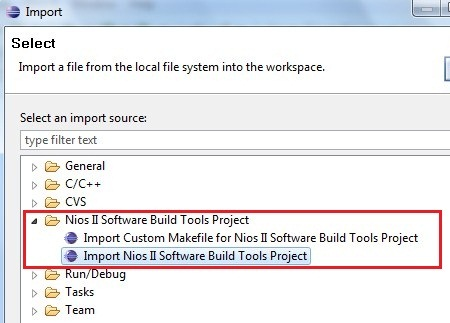
\includegraphics[scale=0.65]{ImportNiosProject}
		\caption{Import Application and BSP files}
		\label{fig:ImportNiosProject}
	\end{figure}
	\begin{figure}[!h]
		\centering
		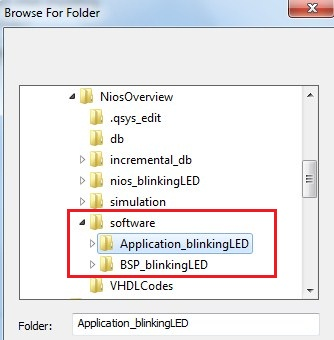
\includegraphics[scale=0.65]{LocationProject}
		\caption{Application and BSP files are in software folder}
		\label{fig:LocationProject}
	\end{figure}
	\begin{figure}[!h]
		\centering
		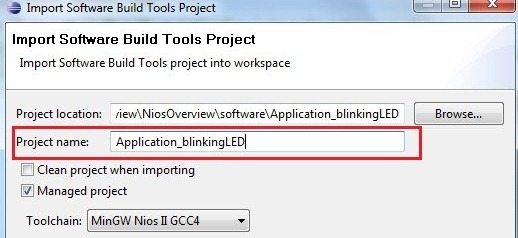
\includegraphics[scale=0.5]{ApplicationAdded}
		\caption{Add application Name i.e. Application\_blinkingLED}
		\label{fig:ApplicationAdded}
	\end{figure}
	\item Similarly, add the BSP folder in the current workspace. 
	\item Now, open the `system.h' file in the BSP. Here, we can see that LED data width is still `1' as shown in Fig. \ref{fig:noSwitchBeforeUpdateBSP}. Also, we can not find the `switch' entries in the system.h file. 
	\begin{figure}[!h]
		\centering
		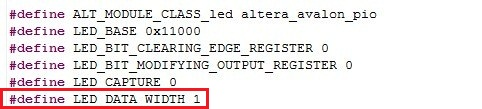
\includegraphics[scale=0.5]{noSwitchBeforeUpdateBSP}
		\caption{LED data width is not updated to `2'}
		\label{fig:noSwitchBeforeUpdateBSP}
	\end{figure}
	\item To update the BSP, right click on the BSP folder and go to Nios$\rightarrow$Generate BSP. It will update the BSP files.
	\item Sometimes, proper addresses are not assigned during generation in `Qsys' system as shown in Fig. \ref{fig:SwitchBaseProblem}. Here, SWITCH\_BASE is set to `0$\times$0'. To remove this problem, assign base addresses again and regenerate the system as discussed in Section \ref{sec:ModifyQysFile}. 
	\begin{figure}[!h]
		\centering
		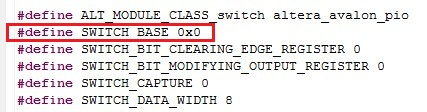
\includegraphics[scale=0.5]{SwitchBaseProblem}
		\caption{Base address is not assigned to switch}
		\label{fig:SwitchBaseProblem}
	\end{figure}	
\end{enumerate} 

\section{Add `C' file for reading switches}
Next, modify the `main.c' file as shown in Listing \ref{c:mainCh2}. Finally, build the system by pressing `ctrl+B'. 

\begin{explanation}[Listing \ref{c:mainCh2}]
	`IORD(base, offset)' command is used the read the values form I/O ports as shown at Line 19 of the listing. Line 19 reads the values of the switches; which is multiply by variable `itr' (see Line 22), to set the delay value base on switch patterns. Also, `iter 'value is set to `1000' at Line 11, so that multiplication can produce sufficient delay to observe the blinking LEDs.
\end{explanation}
\lstinputlisting[
caption    = {Blinking LEDs with C application},
language = C,
label      = {c:mainCh2}
]{CppCodes/main.c}


\section{Simulation and Implementation}
If build is successful, then we can simulate and implement the system as discussed in Chapter \ref{ch:NiosOverview}. Fig. \ref{fig:simulation00} and \ref{fig:simulation01} illustrate the simulation results for switch patterns `0000-0000' and `0000-0001' respectively. Note that, blinking patterns are shown by `01' and `10', which indicates that LEDs will blink alternatively. Also, blinking-time-periods for patterns `0000-0000' and `0000-0001' are `4420 ns' and `1056091 ns' respectively (see square boxes in the figures), which show that blinking periods depend on the switch patterns. 

\begin{figure}[!h]
	\centering
	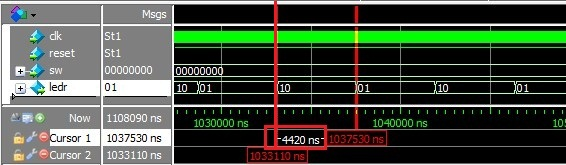
\includegraphics[scale=0.65]{simulation00}
	\caption{Simulation waveforms with switch pattern `0000-0000'}
	\label{fig:simulation00}
\end{figure}
\begin{figure}[!h]
	\centering
	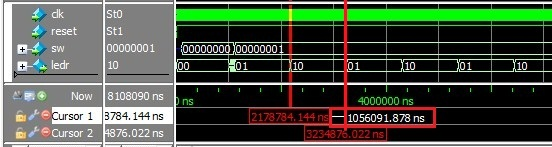
\includegraphics[scale=0.65]{simulation01}
	\caption{Simulation waveforms with switch pattern `0000-0001'}
	\label{fig:simulation01}
\end{figure}	

To implement the design, compile the top level design in Quartus and load the `.sof' file on the FPGA chip. Then load the `.elf' file from Nios software to FPGA chip. After this, we can see the alternatively blinking LEDs on the board. 

\section{Conclusion}
In this chapter, values from the PIO device i.e. switch patterns are read using IORD command. These switch patterns are used to decide the blinking rate of the LEDs. Further, we discussed the procedure to modify the existing Qsys, Quartus and Nios to extend the functionalities of the system. 



